\documentclass[12pt]{extarticle}


\usepackage[utf8]{inputenc}
\usepackage[T2A]{fontenc}      %% 2
\usepackage[english,russian]{babel}    %% 3




\usepackage[square,numbers]{natbib}
\usepackage{setspace}
\usepackage{amssymb}
\usepackage{lipsum}
\usepackage{autonum}
\usepackage{graphicx}
\usepackage{amsmath}
\usepackage{marvosym}

\usepackage{subfig}


\usepackage{float}
\usepackage{booktabs}
\usepackage{xcolor}
\usepackage{hyperref}
\usepackage{comment}
\definecolor{linkcolor}{HTML}{000000} % цвет ссылок
\definecolor{urlcolor}{HTML}{000080} % цвет гиперссылок
\hypersetup{pdfstartview=FitH,  linkcolor=linkcolor,urlcolor=urlcolor, colorlinks=true}
\renewcommand{\baselinestretch}{1.5}
\bibliographystyle{abbrvnat}





 


\begin{document} % начало документа

\section{Введение}

\qquad Квантовые вычисления как самостоятельная область науки появились в 1980-х годах благодаря осознанию возможности реализовывать вычисления на квантовых системах, значительно ускоряя за счёт эффекта квантового параллелизма некоторых трудоёмкие для классического компьютера вычисления. С того времени было предложено множество теоретических квантовых алгоритмов, позволяющих получить полиномиальное, а в определённых случаях экспоненциальное ускорение в сравнении с известными классическими алгоритмами при наличии универсального квантового компьютера. К наиболее известным квантовым алгоритмам можно отнести алгоритм Шора, позволяющий получить экспоненциальное ускорение для задачи факторизации числа и алгоритм Гровера, дающий квадратичное ускорение поиска в неструктурированных базах данных.

\qquad Параллельно с теоретическими открытиями развивались и технологии квантовых компьютеров. На сегодняшний день разработано множество подходов к физической реализации квантовых компьютеров, таких как преобразования над системами фотонов, холодных атомов/ионов в ловушках, квантовых точек или сверхпроводящих цепях. Каждый из перечисленных подходов имеет свои преимущества, при этом ни одна из существующих технологий не позволяет реализовать универсальный квантовый компьютер ввиду ограничений на максимальный размер квантовой системы, максимальный размер полностью запутанной подсистемы и наличии ошибок при реализации преобразований. Доступные на настоящее время способны выполнять преобразования с некоторым уровнем ошибок на небольших квантовых системах. Их принято называть шумными квантовыми устройствами среднего размера (Noisy Intermidiate Scale Quantum англ. NISQ). 

\qquad Прикладное использование таких квантовых алгоритмов, как алгоритм Шора и алгоритм Гровера требует бОльших ресурсов, чем NISQ устройства могут предоставить. Таким образом для практического использования существующих технологий, а так же устройств, которые предположительно появятся в ближайшем будущем, наиболее перспективными представляются гибридные алгоритмы, где часть операций выполняется на классическом компьютере и лишь небольшие подзадачи, сложные для классической обработки выполняются на квантовом устройстве. Гибридные квантово-классические алгоритмы основаны на принципе вариации параметров заданного функционала, поэтом называются вариационными квантовыми алгоритмами (ВКА). ВКА включают в себя различные группы алгоритмов, таких как вариационный квантовый алгоритм нахождения собственных значений операторов ВКС (Variational Quantum Eigensolver англ. VQE) \cite{VQE_review}, квантовый приблизительный оптимизационный алгоритм КПОА (Quantum Approximate Optimization Algorithms англ. QAOA), Квантовые нейросети КНН и тд. 


\qquad В данной работе изучены существующие методы ВКА в приложении к задаче поиска основного состояния квантовых систем, соответствующего минимальной энергии, а так же проведено исследование основных преимуществ и недостатков различных архитектур ВКА. В разделе 1 подробно рассмотрены теоретические аспекты реализации основных алгоритмов ВКА. В пункте 2 представлены методы технической реализации ВКА, подробно рассмотрена проблема аппаратно-эффективной реализации ВКА. Пункт 3 содержит численные результаты сравнения различных вариантов ВКА для решения нескольких задач.

\section{Вариационные Квантовые Алгоритмы}



\subsection{Основные понятия}

\qquad Вариационные Квантовые Алгоритмы (VQA) - гибридные алгоритмы для решения задачи минимизации заданного функционала. На квантовом устройстве реализуется гейтовая схема, состоящая из параметризованной части (анзаца) для приготовления квантового состояния, и  измерительной части, преобразование которой соответствует наблюдаемой, в которую кодируется решаемая задача. На основе оценки наблюдаемой выходного состояния строится функция потерь, минимум которой соответствует решению задачи. Таким образом решение оптимизационной задачи сводится к нахождению набора параметров анзаца для приготовления квантового состояния, минимизирующего функцию потерь, являющуюся функцией квантового состояния и заданной его наблюдаемой.

\qquad Поиск подходящих параметров анзаца проводится с использованием оптимизатора на классическом вычислительном устройстве. Таким образом решение оптимизационной задачи представляет из себя итеративный процесс обновления параметров анзаца в результате взаимодействия квантового устройства с классическим оптимизатором. Схематически процесс работы VQA представлен на Рис.\ref{fig:VQA} и состоит из следующих этапов:

\qquad 0) Кодирование задачи в некоторую наблюдаемую квантового состояния. Представление наблюдаемой в виде системы измерений над квантовым состоянием, реализуемой на квантовом устройстве (например, кодирование в строку матриц Паули):

\begin{equation}
 H=\sum_{i} c_{i} \hat h_{i} = \sum_{i} c_{i} \otimes^{N-1}_{j = 0} \hat \sigma^{j}_{*} 
\end{equation}

, где $\hat h_{i}$ - термы наблюдаемой, отдельно измеряемые на квантовом устройстве, $c_{i}$ - коэффициенты в разложении наблюдаемой на термы, $ \sigma_{*} \in \{\hat I,\hat \sigma_{X}, \hat \sigma_{Y}, \hat \sigma_{Z}  \} $, $\otimes^{N-1}_{j = 0} \hat \sigma^{j}_{*}$ - обозначение произвольной строки матриц Паули длины не более $N$.

\qquad 1) Инициализация параметров анзаца:
Задаётся изначальный набор параметров которые фиксируют определённое состояние квантовых вентилей и тем самым задают определённое преобразование над входным состоянием. $\vec{\theta_{init}}$

\qquad Начало итерационного процесса повторяющегося фиксированное количество шагов или до достижения заданного критерия остановки):

\begin{equation}
i = 0; \psi^{0} = \psi_{init}
\end{equation}

\qquad 2) Приготовление состояния. Входное состояние (обычно $|0 \rangle$) преобразуется анзацем в выходное состояние $|\psi_{i}\rangle$:


\begin{equation}
|\psi^{i}\rangle = |\psi (\vec{\theta^{i}})\rangle = U(\vec{\theta^{i}}) |0 \rangle
\end{equation}



\qquad 3) Измерение. Выходное состояние поступает в фиксированную часть квантовой схемы, где производится набор измерений соответствующий заданной наблюдаемой согласно пункту 0. Данный процесс повторяется многократно для набора статистики и оценки математического ожидания наблюдаемой величины:

\begin{equation}
\lambda(\vec{\theta^{i}}) = \langle \psi(\vec{\theta^{i}}) |H|\psi(\vec{\theta^{i}})\rangle
\end{equation}

, так же для большинства методов оптимизации необходимо произвести дополнительные измерения. Например, для градиентных методов требуется оценка $ \frac{d\lambda(\vec{\theta^{i}})}{d\vec{\theta^{i}}} $, которую можно получить с помощью правила варьирования параметра;

\qquad 4) Обновление параметров анзаца на классическом вычислительном устройстве.
На данном этапе решается классическая задача многомерной оптимизации, целью которой является минимизация заданной функции от вектора параметров с помощью варьирования последних. В зависимости от выбранного метода оптимизации меняется правило обновления параметров. Например при использовании градиентного оптимизатора обновление параметров выглядит следующим образом:
$ \vec{\theta^{i+1}} = \vec{\theta^{i}} - k \nabla_{\mathbf{\theta^{i}}} \lambda(\vec{\theta^{i}})$

\qquad 5) Переход на новую итерацию или завершение оптимизаионного процесса. На данном этапе параметры вариационной схемы обновлены, запускается следующая итерация ВКА. Процесс длится заданное количество итераций, либо останавливается по достижению определённых условий.

\bigskip

\begin{figure}[H]
\center{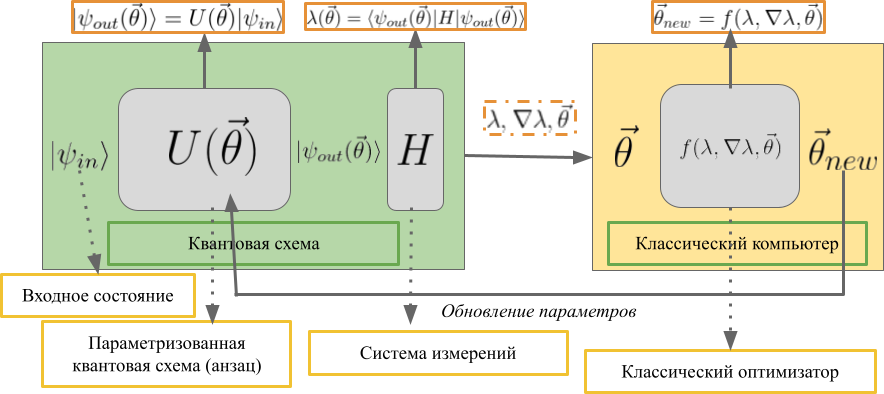
\includegraphics[scale=0.8]{VQA.png}}
\caption{Иллюстрация, поясняющая принцип работы вариационных квантовых алгоритмов.}\label{fig:VQA}
\end{figure}

\bigskip


\subsection{Применение VQA}

\qquad VQA рассматривается в качестве потенциально перспективных алгоритмов для достижения квантового превосходства в проблемах физики многих тел, а так же оптимизационных задачах. Наиболее естественным способом использования VQA является решение задач квантовой химии, таких как исследование статических и динамических свойств молекул и сильно коррелированных электронных систем, которые является фундаментальными задачами во многих областях науки. Например, такие задачи актуальны в биологии для понимания динамики сворачивания белков, в фармацевтике для улучшения возможностей открытия лекарств, в производстве материалов для изучения высокотемпературной сверхпроводимости. В ядерной физике VQA так же могут найти аналогичные применения для исследования энергетической структуры ядра частиц. 

\qquad Второй потенциальной областью применения VQA являются проблемы оптимизации. Предпосылкой является возможность использования высокой размерности гильбертова пространства для кодирования оптимизационных проблем с надеждой на ускорение решения за счёт наличия квантовой запутанности кубитов ВКА. Одним из лидирующих кандидатов на достижение квантового превосходства признаются класс VQA называемый QAOA, предназначенный для решения классических комбинаторных задач. В основе таких предположений заложен то факт, что даже при наиболее простой параметризации анзац QAOA алгоритмов не поддаётся эффективному моделированию на классическом компьютере, что открывает новые возможности для решения оптимизационных проблем.

\qquad Так же в отдельную область можно выделить применение VQA в задачах машинного обучения. Наиболее перспективными алгоритмами в области Квантового Машинного Обучения (QML) на данный момент считаются квантовые нейронные сети QNN. Для ряда задач показано, что QNN обучаются быстрее аналогичных классических нейронных сетей, а так же отдельный их класс свёрточные квантовые нейронные сети не подвержены проблеме Бесплодных Плато, типичной для ВКА, что открывает большие перспективы для их использования в задачах глубинного обучения, обработки изображений, обучения с подкреплением и тд.

\subsection{Основные трудности и пути решения}

\qquad Несмотря на возможные перспективы VQA в эпоху шумных квантовых устройств средних размеров, их применение до сих пор связано с рядом проблем включая сложность оптимизируемости, точность результатов и эффективность применения VQA в сравнении с классическими алгоритмами.

\qquad Наиболее серьёзной проблемой при оптимизации функции потерь  VQA можно считать наличие феномена называемого бесплодное плато БП. При использовании неструктурированных универсальных анзацев с увеличением размерности решаемой проблемы в среднем частные производные функции потерь экспоненциально быстро стремятся к нулю, другими словами гиперпространство параметров становится практически плоским и для поиска глобального минимума необходимо экспоненциально по размерности пространств долго оптимизироваться случайно блуждая по плоскому участку гиперплоскости, что делает использование VQA неэффективным методом. Возникновение БП в универсальных анзацах можно считать следствием экспоненциального расширения гильбертова пространства оптимизации при углублении анзаца. Так же в серии работ было показано, что возникновение БП может быть вызвано высокой степенью запутанности системы кубитов, а так же наличием шума.

\qquad Так же для достижения квантового преимущества необходимо уметь эффективно проводить измерения с использованием VQA. В общем случае использование подхода VQA не даёт преимущество над чисто классической обработкой в результате недопустимо большого количества измерений, необходимых для оценки наблюдаемых величин. Например, в квантовой химии количество строк Паули в разложении гамильтонианов молекул по термам растёт приблизительно как $~n^{4}$ с ростом количества орбиталей молекулы $n$. В работах ... предложены различные техники с использованием коммутирующих групп операторов измерения для возможности их одновременного измерения и как следствие сокращения общего числа необходимых измерений. 

\qquad Наличие шума в квантовых операциях является ещё одной проблемой использования VQA. Наличие шума приводит к ряду нежелательным последствиям в виде возникновения БП даже в неглубоких схемах, а так же снижению точности результатов в сравнении с оптимизацией в отсутствии шума.


\subsection{Система измерений и функция потерь}

\qquad Первым этапом в решении задачи оптимизации является кодирование минимизируемого функционала в физическую наблюдаемую и её представлении в виде системы измерений над вектором состояния квантовой системы, приготавливаемым с помощью анзаца. В зависимости от поставленной задачи VQA сводятся к алгоритмам VQE (Variational Quantum Eigensolver) или QAOA (Quantum Approximate Optimization Algorithm) отличающимся различными способами кодирования минимизируемого функционала в физическую наблюдаемую.

\qquad Для задач поиска определённых характеристик физической системы используется алгоритм VQE, где в качестве минимизируемого функционала выступает математическое ожидание некоторой физической наблюдаемой по всевозможным состояниям квантовой системы реализуемыми с помощью выбранного анзаца. Например, в задачах квантовой химии для поиска основного состояния молекулы в роли наблюдаемой величины выступает её энергия.

\qquad Наблюдаемая представляется в виде серии измерений в некотором базисе. Удобно в качестве базиса для однокубитовых измерений использовать матрицы Паули $ \{I,\sigma_{X}, \sigma_{Y}, \sigma_{Z}  \}$, тогда наблюдаемая может быть выражена в виде взвешенной суммы строк матриц Паули:

\begin{equation}
\hat H=\sum_{i} c_{i} \hat h_{i} = \sum_{i} \hat c_{i} \otimes^{N-1}_{j = 0} \hat \sigma^{j}_{*} 
\end{equation}

,где $ \sigma_{*} \in \{\hat I,\hat \sigma_{X}, \hat \sigma_{Y}, \hat \sigma_{Z}  \} $, N - размерность системы кубитов;

\qquad Следующим шагом с использованием наблюдаемой составляется функция потерь, минимум которой совпадает с заданным функционалом. В простейшем случае функция равняется математическому ожиданию наблюдаемой:

\begin{equation}
 C( \vec \theta, \hat H ) = \langle \hat H \rangle = \sum_{i} c_{i} \langle \hat h_{i} \rangle
\end{equation} 

\qquad При этом в качестве функции потерь можно выбрать и другую функцию от вектора параметров $\theta$ и оператора наблюдаемой $\hat H$ с совпадающим минимум. Например, для части задач эффективно использование в качестве функции потерь энергии Гиббса:

\begin{equation}
 C( \vec \theta, \hat H ) = G = -ln \langle \exp^{-\eta \hat H} \rangle
\end{equation} 

\qquad В некоторых специфических областях применения VQA, таких как квантовая коррекция ошибок, квантовая метрология, вариационное решение линейных уравнений и тд., функция потерь может быть представлена принципиально другим образом. Более того в некоторых случаях представляется возможность задать локальную функцию потерь, вместо глобальной ( оцениваются только однокубитовые наблюдаемые и потом суммируются, в отличие от глобальной функции потерь, где оценивается наблюдаемая, действующая на полное состояние квантовой системы). Доказано, что локальные функции потерь меньше подвержены возникновению БП и соответственно значительно более эффективны в использовании.

\qquad В задачах комбинаторной оптимизации стандартным способом применения VQA является QAOA, который по сути представляет из себя троттеризированную аналогию квантового адиабатического перехода из основного состояния, соответствующего гамильтониану $H_{M}$ в основное состояние гамильтониана, соответствующего проблеме $H_{P}$. Функция $f(e_{i})$ в QAOA кодирует комбинаторную проблему в средние значения в базисе битовых строк (векторов состояний). Тогда гамильтониан, соответствующий проблеме может быть представлен в виде:
 

\begin{equation}
H_{P} = \sum^{n}_{i=1} f(e_{i}) | e_{i} \rangle \langle e_{i} |
\end{equation}

\qquad При этом гамильтониан изначального суперпозиционного состояния представляет из себя:

\begin{equation}
H_{M} = \sum^{n}_{i=1} \hat{ \sigma^{i}_{x} }
\end{equation}

\qquad А само начальное состояние представляет из себя равновероятную суперпозицию всех базисных векторов и выражается формулой:

\begin{equation}
|D \rangle = \frac{1}{\sqrt{2^{n}}} \sum^{n}_{i = 0} |e_{i} \rangle
\end{equation}

\qquad В результате анзац QAOA способствует эволюции начального состояния $|D \rangle $ под переменным действием гамильтонианов $H_{M}$ и $H_{P}$ и выходное состояние записывается в виде: 

\begin{equation}
| \Psi(\gamma, \beta) \rangle =  \exp^{-i \beta_P H_M} \exp^{-i \gamma_P H_P} \cdots \exp^{-i \beta_1 H_M} \exp^{-i \gamma_1 H_P}|D \rangle
\end{equation} 

\qquad А функция потерь записывается в виде мат ожидания наблюдаемой, соответствующей проблеме, по параметризованному выходному состоянию:

\begin{equation}
C(\gamma, \beta) = \langle \Psi(\gamma, \beta)  | H_{P} | \Psi(\gamma, \beta) \rangle
\end{equation} 

\qquad И итоговая задача сводится к минимизации функции потерь $ min_{\gamma, \beta} (C(\gamma, \beta))$.


\qquad  

\subsection{Анзац}

\qquad Анзац VQA, как отмечалось выше, представляет из себя параметризованную квантовую схему, которое готовит различные в зависимости от параметризации состояния системы в поисках состояния, минимизирующего значение наблюдаемой. В общем случае анзац может быть представлен в виде слоистой структуры, тогда преобразование над входным состоянием можно записать в следующем виде:

\begin{equation}
U(\vec \theta) = U_{L}(\vec \theta_{L}) \cdots U_{2}(\vec \theta_{2}) U_{1}(\vec \theta_{1})
\end{equation}

, где 

\begin{equation}
U_{l}(\vec \theta_{l}) = \prod_{m} e^{-i \theta_{m} H_{m} } W_{m}
\end{equation} , где $W_{m}$ - непараметрическое унитарное преобразование, а $Н_{m}$ - эрмитов оператор



\qquad Выбор анзаца VQA чрезвычайно важен для эффективной работы алгоритма, так как именно анзац задаёт пространство $U$ возможных преобразований над состоянием квантовой системы и как результат пространство выходных состояний $\Psi$. В основном для описания анзаца используются такие его характеристики, как выразительность ( и средняя мера запутанности выходных состояний.

\qquad Выразительность анзаца описывает универсальность преобразований, которые можно получить варьирую его параметры. Таким образом максимально выразительный анзац с равной вероятностью совершает произвольное унитарное преобразование над квантовым состоянием. Для количественной оценки выразительности анзаца используется сравнение распределения состояний полученных на выходе рандомно инициализированного анзаца $U(\vec \theta)$ с максимально выразительным распределением квантовых состояний, распределением Хаара. Описанная мера выразительности называется мерой Хаара и для $t$ - го момента описывается формулой:

\begin{equation}
A^{(t)}(U) = \int dU_{Haar}U^{\otimes t}_{Haar} |0 \rangle |0 \langle 0 | {(U^{\dagger}_{Haar})}^{\otimes t} - \int dU U^{\otimes t} |0 \rangle |0 \langle 0 | {(U^{\dagger})}^{\otimes t}
\end{equation}

\qquad Для возможности использования выбранного анзаца для решения задачи необходимо, чтобы анзац был достаточно выразителен чтобы приготовить состояние соответствующее решению задачи $\psi_{target} \in \Psi_{ansatz} $. При этом высокая выразительность анзаца обычно является отрицательным фактором, так как значительно усложняет поиск глобального минимума функции потерь. В частности высокая выразительность анзаца связана с появлением БП, так как гильбертовом пространств оптимизации  экспоненциально растёт с увеличением размерности системы.

\qquad Так же было показано, что помимо большой выразительности анзаца причиной появления БП может стать высокая запутанность состояния приготавливаемого анзацем. Таким образом анзацы с высокой средней запутанностью выходного состояния с большой вероятностью подвержены возникновению БП.

\qquad Существует два основных подхода к реализации анзаца. Первый называется аппаратно-эффективным и заключается в использовании универсального анзаца, элементы и архитектура которого легко реализуется на выбранном квантовом устройстве. Такой подход перспективен в первую очередь ввиду его универсальности и простоты реализации. Особенно эффективно применение к Гамильтонианам схожей структуры с архитектурой анзаца. При этом Аппаратно-эффективный универсальный анзац приводит к сложностям в оптимизации и возникновению БП в связи с высокой выразительностью анзаца и запутанностью выходного состояния. В ряде случаев данную проблему помогает избежать эффективная инициализация начальных параметров.

\qquad Второй подход основан на идее использования информации о решаемой проблеме для построения архитектуры анзаца, получая в результате "вдохновлённую проблемой" архитектуру анзаца. Такой подход позволяет сильно сократить выразительность анзаца, значительно ускоряя процесс оптимизации, и снижая вероятность появления БП, при этом гарантируя достижимость состояния минимизирующего наблюдаемую.

\subsection{Инициализация параметров} 

\qquad Процесс оптимизации параметризованной схемы VQA начинается с инициализации параметров. Случайная инициализация параметров, особенно в универсальных анзацах, зачастую приводит к застревании процесса оптимизации на БП. При этом правильно выбранные начальные параметры могут помочь оптимизатору не попасть в БП, даже для анзацев, в которых таковое имеется.

\qquad В литературе рассматривается множество подходов к эффективной инициализации начальных параметров. Например, в статье ... предлагается оптимизировать анзац слой за слоем, чтобы при добавлении нового слоя с большой вероятностью вектор параметров соответствовал точке в пространстве оптимизации, близкой к глобальному минимуму частичного анзаца, что позволяет оптимизатору избежать БП и достигнуть глобального минимума полного анзаца. В работе ... предлагается разбить слоистый анзац на $D$ блоков по $2K$ слоёв и инициализировать в каждом блоке первые $K$ слоёв случайно, а последующие так чтобы каждый блок в результате давал единичное преобразование:

\begin{multline}
U(\vec \theta_{init}) = [U_{L}(\vec \theta_{L}) \cdots U_{L-K}(\vec \theta_{L-K}) U^{\dagger}_{L-K-1}(\vec \theta_{L-K-1} U^{\dagger}_{L-2K}(\vec \theta_{L-2K})]  \cdots \\ 
[U_{2K}(\vec \theta_{2K}) \cdots U_{K}(\vec \theta_{K}) U^{\dagger}_{K-1}(\vec \theta_{K-1} U^{\dagger}_{0}(\vec \theta_{0})] =  \\  U^{*}_{D}(\vec  \theta_{L} \cdots \vec  \theta_{L-2K}) \cdots U^{*}_{0}(\vec \theta_{2K} \cdots \vec  \theta_{0}) =  I_{D} \cdots I_{0} = I
\end{multline}

\qquad Инициализация единичными блоками даёт возможность рассматривать анзац на первых шагах, как неглубокий и с малой степенью запутанности, гарантируя инициализацию начальных параметров на некотором отдалении от БП. 

\subsection{Классический оптимизатор}

\qquad Классический оптимизатор итеративно обновляет параметры анзаца для достижения минимального значения функции потерь, заданной в виде математического ожидания значения наблюдаемой квантовой системы $min ( \langle \psi(\vec{\theta_{init}}) |H|\psi(\vec{\theta_{init}})\rangle )$. На каждой итерации на вход оптимизатор принимает вектор параметров $\vec \theta_{in} $, значение функции потерь при заданном векторе  параметров $С(\vec \theta_{in}) $, а так же дополнительные характеристики в зависимости от метода,далее вычисляется обновлённый вектор параметров $\vec \theta_{out} $ и передаётся на квантовое устройство для перехода на следующую итерацию.

\qquad Оптимизаторы делятся на градиентные и безградиентные по принципу обновления параметров. Оптимизационные методы не использующие градиент в основном являются эвристическими. Такие методы оптимизации основаны на естественных процессах, приводящих к оптимальным результатам. К безградиентным методам относятся генетические алгоритмы, основанные на селекции оптимальных качеств в ходе естественного отбора, алгоритм роя частиц, основанный на поведении стадных животных для достижения оптимальных условий, алгоритм симуляции отжига, основанный на минимизации энергии кристаллической решётки металла в процессе закалки ("отжига").

\qquad Градиентные методы используют принципиально другой подход к оптимизации. Итеративное обновление параметров в общем виде происходит по методу градиентного спуска согласно следующей формуле:

\begin{equation}
\vec{\theta_{out}} = \vec{\theta_{in}} - k \frac{dС(\vec{\theta_{in}})}{d\vec{\theta_{in}}}
\end{equation}

\qquad Заметим, что градиент функции потерь рассчитывается также на квантовом устройстве. Стандартным способом оценки частной производной функции потерь на квантовом устройстве является PSR (Parameter Shift Rule):

\begin{equation}
 \frac{\partial  \lambda (\vec \theta)}{\partial \theta_{i}} = \frac{ \lambda (\theta_{0},..., \theta{i} + \pi/2, ..., \theta_{K}) - \lambda (\theta_{0},..., \theta{i} - \pi/2, ..., \theta_{K})}{2}
\end{equation}

\qquad Оценка градиента получается использованием PSR за $2T$ запусков, где $T$ - размерность вектора параметров $\vec \theta$. 

\qquad Существует множество модификаций градиентного спуска, увеличивающих скорость сходимости и точность результата, способствуя выходу из локальных минимумов. Одним из наиболее популярных оптимизаторов в классическом машинном обучении, где также необходимо решать задачи оптимизации высокой размерности, является ADAM (ADAptive Moment estimation). Данный алгоритм способствует выходу из локальных минимумов за счёт наличия инерции в оценке градиента на новой итерации, а так же учитывает важность оптимизации по каждому из параметров, оценивая накопительную дисперсию. Алгоритм обновления параметров методом ADAM выглядит следующим образом:

\begin{equation}
x^{(t+1)} = x^{(t)} - \eta^{(t+1)} \frac{a^{(t+1)} }{   \sqrt{b^{(t+1)}} + \epsilon}
\end{equation}

, где $a^{(t+1)}$ накопительная оценка градиента на $t+1$ итерации, $b^{(t+1)}$ накопительная оценка нецентрированной дисперсии на $t+1$ шаге, $\eta^{(t+1)}$ - нормировочный коэффициент на $t+1$ шаге;

\qquad Существуют так же градиентные методы, требующие дополнительной информации о функции потерь. На данный момент одним из ведущих таких методов, который возможно реализовать на гибридном устройстве является QNG (Quantum Natural Gradient). Обыкновенный градиентный спуск на каждом шаге использует градиент функции потерь в Евклидовом пространстве, но в случае VQA пространство оптимизации не является Евклидовым. QNG учитывает неевклидовость пространства оптимизации с помощью умножения градиента функции на Fubini-Study метрический тензор который оценивается на квантовом устройстве каждом шаге $t$ - му шагу, в результате чего оперирует с оценкой градиента функции потерь в Римановом пространстве.


\begin{equation}
x^{(t+1)} = x^{(t)} - \eta g ( f( x^{(t)} )  )^{-1} \nabla f( x^{(t)}  )
\end{equation}

, где $g ( f( x^{(t)} )  )$ - метрический тензор функции потерь в точке соответствующей вектору параметров на $t$ шаге;

\qquad Оценка метрического тензора проводится на квантовом устройстве согласно следующему выражению:

\begin{equation}
g_{ij}^{(l)} = \langle \psi_{l} | K_{i}K_{j} |\psi_{l}  \rangle - \langle \psi_{l} | K_{i} | \rangle  \langle \psi_{l} | K_{j} |\psi_{l}  \rangle 
\end{equation}

, где $K^{(l)}_{i}$ - генератор $i$-го квантового вентиля на $l$-м слое анзаца.

\qquad Таким образом реализация QNG на квантовом устройстве с оценкой градиента с помощью parameter-shift rule для анзаца с $L$ слоями и $T$ параметрами требуется провести $E = 2T + L$ оценок на каждом шаге оптимизации. Заметим, что для неглубоких анзацев большой размерности $L<<T$, следовательно количеств дополнительных необходимых измерений незначительно в сравнении со стандартным градиентным спуском ($2T + L ~ 2T$).



\section{Техническая реализация VQA}
\subsection{Блочный анзац}

\section{Моделирование VQA, численные расчеты}
\subsection{Инструменты анализа эффективности}
\subsection{Выбор метода оптимизации}
\subsection{Гамильтониан Швингера}
\subsection{Квантовая химия}



\section{Выводы}


\begin{comment}

	\begin{center}
	\textbf{\Large{���������� ��������������� ����������� ����� �.�. ����������}} \\
		\vspace{4em}
		\textbf{\Large{���������� ���������}} \\
		\vspace{4em}
		\textbf{\Large{������� ��������� �����������}} 
			\vspace{4em}
		
	\end{center}
	

	
	\vspace{12em}
	
	\begin{center}
		\textbf{\LARGE{������� ���������-����������� ����� ��� ������������ ��������� ����������}}
	\end{center}
	
	\vspace{2em}
	
	\begin{center}
		\large{��������� ������ �������� ������ 227�� \linebreak
		 ���������� ���������� ���������}
	\end{center}
	
	\vspace{6em}
	
	\begin{flushleft}
		
	\large{	������� ������������ \linebreak
	
	�.�.-�.�., �.�.�. ������ ��������� ���������� \linebreak
	 ����������� ���������� ��� ����� �.�. ���������� \linebreak 
	 ������ ������ �������}\\
		\vspace{1.5em}
	
	
	\end{flushleft}
	
	\vspace{\fill}
	
	\begin{center}
	\textbf{{\large ������ 2022}}
	\end{center}
	\thispagestyle{empty} 

\end{comment}

\bibliography{library}
\section{Приложение}

\end{document}